%------------------------------------------------------------------------
%Editar Diplomado
\hypertarget{cv:modificarPaso}{\section{Modificar Paso}} \label{sec:modificarPaso}

	Esta funcionalidad le permitirá modificar la información de un paso previamente registrado con el fin de corregir o actualizar datos del mismo. 

		\subsection{Procedimiento}

			%Pasos de procedimiento
			\begin{enumerate}
	
			\item Oprima el botón \IUEditar{} de algún registro existente de la pantalla \ref{fig:GestionarPasos} ''Gestionar Pasos''.
	
			\item Se mostrará la pantalla \ref{fig:modificarPaso} ''Modificar Paso''.
			
			%Pantalla
			\begin{figure}[htbp!]
				\begin{center}
					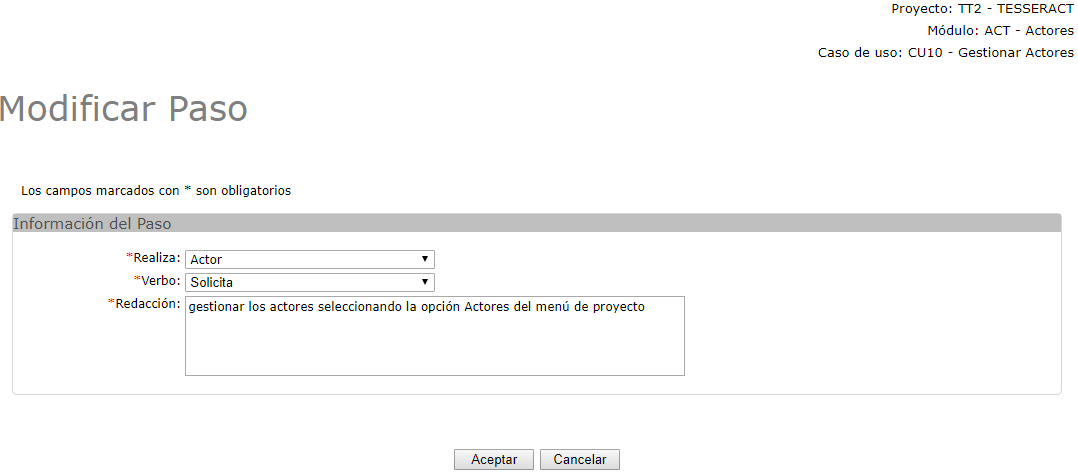
\includegraphics[scale=0.6]{roles/lider/casosUso/trayectorias/pasos/pantallas/IU6-1-1-1-2modificarPaso}
					\caption{Modificar Paso}
					\label{fig:modificarPaso}
				\end{center}
			\end{figure}
		
			\item Modifique los datos solicitados por la pantalla.
			
			\item En la redacción usted podrá referenciar todos los tipos de elementos que se encuentren registrados dentro del proyecto actual, mendiante los siguientes TOKENS:
			
			\begin{itemize}
				\item Podrá referenciar elementos de tipo actor con el TOKEN: ''ACT·''.
				\item Podrá referenciar elementos de tipo entidad y/o atributos con los TOKEN: ''ENT·''y ''ATR·''.
				\item Podrá referenciar elementos de tipo regla de negocio con el TOKEN: ''RN·''.
				\item Podrá referenciar elementos de tipo caso de uso con el TOKEN: ''CU·''.
				\item Podrá referenciar elementos de tipo pantalla con el TOKEN: ''IU·''.
				\item Podrá referenciar elementos de tipo acción con el TOKEN: ''ACC·''.
				\item Podrá referenciar elementos de tipo mensaje con el TOKEN: 'MSG·''.
				\item Podrá referenciar elementos de tipo término con el TOKEN: ''GLS·''.
				\item Podrá referenciar elementos de tipo trayectoria con el TOKEN: ''TRAY·''.
				\item Podrá referenciar elementos de tipo paso con el TOKEN: ''P·''.
			\end{itemize}
						
			\item Oprima el botón \IUAceptar.
			
			\item Se mostrará el mensaje \ref{fig:pasoModificado} en la pantalla \ref{fig:GestionarPasos} ''Gestionar Pasos''.
			
			\begin{figure}[htbp!]
				\begin{center}
					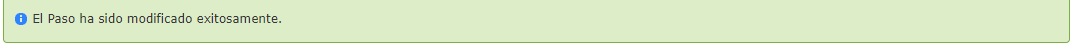
\includegraphics[scale=0.6]{roles/lider/casosUso/trayectorias/pasos/pantallas/IU6-1-1-1-2MSG1}
					\caption{MSG: Paso Actualizado}
					\label{fig:pasoModificado}
				\end{center}
			\end{figure}
			\end{enumerate}